% Provenance (never printed): old premiere S material on subduction (Wadati-Benioff
% planes, density of the old lithosphere, slab pull, transformation of the slab at
% depth: blueschist and eclogite; anatomy of an active margin). Sections from
% figdata/grade-11/slab_sections.py (USGS ComCat M >= 6 1976-2025, PB2002 steps,
% Seton 2020 ages); plate speeds from plate_velocities.py (NNR-MORVEL56 RMS).
% Metamorphism is defined in g12.03, the volcanic arc in g12.04: named only here.
\chapter{क्षेपण क्षेत्र}\label{ch:g11:subduction-zones}

दक्षिण-पश्चिमी प्रशांत में टोंगा द्वीपों के नीचे पृथ्वी कहीं और की अपेक्षा
कहीं अधिक गहराई पर काँपती है। 1976 और 2025 के बीच संसार भर में दर्ज
परिमाण 6 या उससे अधिक के सात हज़ार भूकंपों में से सबसे गहरा
\qty{688}{km} नीचे हुआ, और इस अध्याय में टोंगा के आर-पार की काट में लगभग \qty{671}{km} तक
की घटनाएँ हैं। ऐसी गहराइयों पर चट्टान गरम और भारी
दाब में होती है; उसे \omterm{def:g11:lithosphere-asthenosphere:lithosphere}{दुर्बलतामंडल} की तरह धीरे-धीरे बहना चाहिए, टूटना नहीं। फिर भी वह
टूटती है। यह अध्याय समझाता है कि वहाँ टूटने के लिए क्या है: ठंडी महासागरीय
तली की एक \omterm{def:g11:subduction-zones:slab}{स्लैब}, जो वापस प्रावार में डूब रही है।
% ledger: data:usgs-comcat (catalogue_maxdepth 688; tonga_maxdepth 670.8, slab_sections.py)

\begin{recall}
किसी अभिसारी सीमा पर दो प्लेटें एक-दूसरे की ओर चलती हैं; उनमें से कुछ के अनुदिश
गहरी खाइयाँ होती हैं (पुस्तक 1, कक्षा 7 और 8)। भूकंप का परिमाण
उसका आकार मापता है, और समुद्र के नीचे का भूकंप सुनामी उठा सकता है
(पुस्तक 1, कक्षा 7)। किसी प्लेट का दूसरी के सापेक्ष वेग उनके वेगों का
अंतर है (\cref{ch:g11:plate-motions})। महासागरीय तली
आयु के साथ धँसती है, और लगभग 60 मिलियन वर्ष बाद उसका \omterm{def:g11:lithosphere-asthenosphere:lithosphere}{स्थलमंडल}, लगभग
\qty{100}{km} मोटा, अपने नीचे के \omterm{def:g11:lithosphere-asthenosphere:lithosphere}{दुर्बलतामंडल} से अधिक घना होता है
(\cref{ch:g11:ocean-ridges})। भूकंपीय तरंगें प्रावार में लगभग \qty{670}{km} पर
एक तीव्र परिवर्तन दिखाती हैं (\cref{ch:g11:seismic-structure})। कायांतरित चट्टान
ठोस अवस्था में रूपांतरित चट्टान है (पुस्तक 1, कक्षा 6)।
\end{recall}
% ledger: data:prem (670 km), ps77:depth-age

\section{खाइयाँ और झुके हुए भूकंप-क्षेत्र}

अधिकांश भूकंप उथले होते हैं: 1976 से परिमाण 6 या उससे अधिक की सूची में
केवल लगभग पाँच में से एक \qty{70}{km} से अधिक गहरा है, और पंद्रह में से एक
\qty{300}{km} से अधिक गहरा। नीचे का मानचित्र दिखाता है कि गहरे भूकंप कहाँ हैं।
% values (slab_sections.py): frac_deeper_70 0.21, frac_deeper_300 0.069; data:usgs-comcat

\begin{omfigure}
\begin{tikzpicture}
\begin{axis}[ommap, width=\linewidth, xtick={-180,-90,...,180}, ytick={-60,0,60},
  legend style={font=\scriptsize, at={(0.5,-0.13)}, anchor=north, legend columns=3,
    /tikz/every even column/.append style={column sep=6pt}}]
\addplot[fill=omLithAlluv, draw=black!45, line width=0.2pt, forget plot] table {figdata/out/shared-geo-land.dat};
\addplot[black!70, line width=0.5pt, forget plot] table {figdata/out/shared-geo-school-subduction.dat};
\addplot[fill=black!70, draw=none, forget plot] table {figdata/out/shared-geo-school-teeth.dat};
% computed in figdata/grade-11/slab_sections.py; ledger: data:usgs-comcat, data:pb2002
\addplot[only marks, mark=*, mark size=0.55pt, black!45] table[x=lon, y=lat] {figdata/out/grade-11-slab_sections-world-shallow.dat};
\addplot[only marks, mark=*, mark size=0.8pt, omProp] table[x=lon, y=lat] {figdata/out/grade-11-slab_sections-world-mid.dat};
\addplot[only marks, mark=*, mark size=1.1pt, omThm] table[x=lon, y=lat] {figdata/out/grade-11-slab_sections-world-deep.dat};
\legend{{\qty{70}{km} से उथले}, {70 से \qty{300}{km}}, {\qty{300}{km} से गहरे}}
\end{axis}
\end{tikzpicture}

{\small परिमाण 6.5 या उससे अधिक के भूकंप, 1976--2025 (2192 घटनाएँ),
गहराई के अनुसार रंगे हुए, खाइयों के साथ (काली रेखा, त्रिभुज ऊपर चढ़ने वाली
प्लेट पर)। मध्यवर्ती और गहरे भूकंप केवल कुछ खाइयों के अनुदिश हैं,
हमेशा ऊपरी प्लेट की ओर। आँकड़े: USGS भूकंप-सूची;
प्लेट-सीमाएँ बर्ड (2003) से; स्थल नैचुरल अर्थ से।}
\end{omfigure}
% values: world_n_m65 2192, world_deep_n 197 (slab_sections.py)

गहरे भूकंप बिखरे नहीं हैं: वे पश्चिमी प्रशांत की खाइयों का अनुसरण करते हैं,
कामचटका से जापान, मारियाना, इंडोनेशिया और टोंगा तक,
और दक्षिण अमेरिका के पश्चिमी तट के अनुदिश की खाई का; और वे हमेशा खाई की
एक ओर होते हैं, उस प्लेट के नीचे जो नहीं डूबती।

\begin{definition}[क्षेपण; क्षेपण क्षेत्र]\label{def:g11:subduction-zones:subduction}
\emph{क्षेपण}\index{क्षेपण} \omterm{def:g11:ocean-ridges:oceanic-lithosphere}{महासागरीय स्थलमंडल} की किसी प्लेट का
किसी दूसरी प्लेट के नीचे, वापस प्रावार में, डूबना है। \emph{क्षेपण
क्षेत्र}\index{क्षेपण क्षेत्र} ऐसी अभिसारी प्लेट-सीमा है जहाँ क्षेपण
होता है; सतह पर इसे एक खाई चिह्नित करती है।
\end{definition}

\begin{definition}[वादाती--बेनिऑफ़ क्षेत्र]\label{def:g11:subduction-zones:benioff}
\emph{वादाती--बेनिऑफ़ क्षेत्र}\index{वादाती--बेनिऑफ़ क्षेत्र} भूकंपों की वह झुकी हुई
पट्टी है जो किसी खाई से शुरू होकर ऊपरी प्लेट के नीचे अधिकाधिक
गहरी जाती है, लगभग \qty{700}{km} तक।
\end{definition}
% ledger: frohlich87:wadati

\begin{history}[वादाती और बेनिऑफ़]
1920 के दशक में प्रमुख भूकंपविज्ञानियों का तर्क था कि भूकंप केवल
पहले कुछ दसियों किलोमीटर में हो सकते हैं: उनका तर्क था कि अधिक गहरी पृथ्वी में
विकृति संचित करने की शक्ति नहीं है। जापानी भूकंपविज्ञानी कियू वादाती ने, जो
जापान मौसमविज्ञान एजेंसी के स्टेशनों के सघन जाल के साथ काम करते थे, 1928 से
पहला विश्वसनीय प्रमाण दिया कि कुछ भूकंप सैकड़ों
किलोमीटर गहरे होते हैं: उनके द्वारा अध्ययन की गई घटनाओं में से एक, जनवरी 1927 की,
\qty{420}{km} नीचे थी। 1935 में उन्होंने इन भूकंपों की गहराइयों का पहला
मानचित्र प्रकाशित किया, समोच्च रेखाओं के रूप में खींचा हुआ, और देखा कि गहरा होता
क्षेत्र सक्रिय ज्वालामुखियों की पंक्ति के समांतर चलता था। 1949 और 1954 में
अमेरिकी भूकंपविज्ञानी ह्यूगो बेनिऑफ़ ने दिखाया कि एंडीज़ और
टोंगा--केरमाडेक द्वीपों के नीचे भूकंप ऐसे क्षेत्रों के अनुदिश हैं जो लगभग
\qty{700}{km} की गहराई तक पहुँचते हैं। इन क्षेत्रों को पहले, 1967 में, बेनिऑफ़ क्षेत्र कहा गया;
\omterm{def:g11:subduction-zones:benioff}{वादाती--बेनिऑफ़ क्षेत्र} नाम, जो दोनों को उनका श्रेय देता है, 1971 में
जापानी भूभौतिकविद सेइया उयेदा के एक सुझाव से आया।
\end{history}
% ledger: frohlich87:wadati

\begin{method}[भूकंप-काट को पढ़ना]\label{met:g11:subduction-zones:section}
\begin{enumerate}
  \item खाई के लंबवत, खाई से ऊपरी प्लेट की ओर, एक रेखा
        चुनिए, और उसकी दोनों ओर की एक पट्टी के भीतर के भूकंप
        रखिए।
  \item हर भूकंप को रेखा के अनुदिश उसकी दूरी पर (क्षैतिज रूप से)
        और उसकी गहराई पर (ऊर्ध्वाधर रूप से, नीचे की ओर) आलेखित कीजिए।
  \item झुकी हुई पट्टी देखिए; वह सरल रेखा खींचिए जो उसका सबसे अच्छा
        अनुसरण करती है।
  \item रेखा के दो बिंदुओं से पट्टी का नमन पढ़िए (नीचे का
        प्रस्ताव)।
\end{enumerate}
\end{method}

\begin{omfigure}
\begin{tikzpicture}
\begin{axis}[omrecord, omdepth, name=tonga, width=0.5\linewidth, height=6.4cm,
  xmin=-150, xmax=900, ymin=0, ymax=720, xlabel={खाई से दूरी (\unit{km})},
  ylabel={गहराई (\unit{km})}, title={\small टोंगा}, clip=false]
% computed in figdata/grade-11/slab_sections.py; ledger: data:usgs-comcat, data:pb2002
\addplot[only marks, mark=*, mark size=1.2pt, black!65] table[x=x, y=depth] {figdata/out/grade-11-slab_sections-tonga.dat};
\addplot[omProp, line width=1pt, domain=135.7:761.6, samples=2] {-23.568 + 0.91068*x};
\addplot[only marks, mark=triangle*, mark size=3pt, omDef] coordinates {(0,0)};
\node[font=\scriptsize, anchor=south west, text=omDef] at (axis cs:10,8) {खाई};
\node[font=\scriptsize, anchor=west, text=omProp, align=left] at (axis cs:300,560) {नमन\\\ang{42}};
\end{axis}
\begin{axis}[omrecord, omdepth, at={(tonga.east)}, anchor=west, xshift=0.3cm, width=0.5\linewidth, height=6.4cm,
  xmin=-150, xmax=900, ymin=0, ymax=720, xlabel={खाई से दूरी (\unit{km})},
  yticklabels={}, title={\small एंडीज़, \ang{21} दक्षिण के पास}, clip=false]
\addplot[only marks, mark=*, mark size=1.2pt, black!65] table[x=x, y=depth] {figdata/out/grade-11-slab_sections-andes.dat};
\addplot[omProp, line width=1pt, domain=253.0:900, samples=2] {-88.745 + 0.74613*x};
\addplot[only marks, mark=triangle*, mark size=3pt, omDef] coordinates {(0,0)};
\node[font=\scriptsize, anchor=south west, text=omDef] at (axis cs:10,8) {खाई};
\node[font=\scriptsize, anchor=west, text=omProp, align=left] at (axis cs:300,560) {नमन\\\ang{37}};
\end{axis}
\end{tikzpicture}

{\small दो खाइयों के लंबवत भूकंप-काटें: परिमाण 6 या उससे अधिक के भूकंप,
1976--2025, काट-रेखा से \qty{150}{km} के भीतर,
खाई से उनकी दूरी (ऊपरी प्लेट की ओर) और
उनकी गहराई पर आलेखित। नारंगी: वह सरल रेखा जो 100 और \qty{600}{km} गहराई के बीच के
भूकंपों का सबसे अच्छा अनुसरण करती है। टोंगा के नीचे पट्टी
\qty{670}{km} से नीचे तक पहुँचती है। आँकड़े: USGS भूकंप-सूची; खाइयों की स्थितियाँ बर्ड (2003) से।}
\end{omfigure}
% values (slab_sections.py): tonga_dip 42.3, fit -23.568 + 0.91068 x (77 events);
% andes_dip 36.7, fit -88.745 + 0.74613 x; trench points tonga (-173.31, -20.395),
% andes (-71.286, -21.01)

\begin{proposition}[भूकंप-काट से स्लैब का नमन]\label{prop:g11:subduction-zones:dip}
यदि \omterm{def:g11:subduction-zones:benioff}{वादाती--बेनिऑफ़ क्षेत्र} का अनुसरण करने वाली रेखा के दो बिंदु खाई से
क्षैतिज दूरियों $x_1 < x_2$ पर और गहराइयों $z_1$ और $z_2$ पर हैं,
तो उसका नमन $\delta$, यानी क्षैतिज से उसका कोण, यह संतुष्ट करता है:
\[
  \tan \delta = \frac{z_2 - z_1}{x_2 - x_1}.
\]
\end{proposition}

\begin{proof}
दोनों बिंदु और दूसरे बिंदु के ठीक ऊपर गहराई $z_1$ पर स्थित बिंदु
एक समकोण त्रिभुज बनाते हैं। उसकी क्षैतिज भुजा $x_2 - x_1$ है, उसकी ऊर्ध्वाधर भुजा
$z_2 - z_1$, और पहले बिंदु पर का कोण नमन है। समकोण त्रिभुज के किसी
कोण की स्पर्शज्या सम्मुख भुजा बटा आसन्न भुजा है।
\end{proof}

\begin{example}[टोंगा के नीचे नमन]\label{ex:g11:subduction-zones:dip}
टोंगा काट की रेखा खाई से \qty{300}{km} पर \qty{250}{km} नीचे से
और \qty{700}{km} पर \qty{614}{km} नीचे से गुज़रती है। इसलिए
$\tan\delta = (614 - 250)/(700 - 300) = 364/400 = 0.91$, और
$\delta \approx \ang{42}$। एंडीज़ के नीचे, \ang{21}~दक्षिण पर, यही
विधि लगभग \ang{37} देती है।
\end{example}
% values: tonga line at 300 km 249.6, at 700 km 613.9 (slab_sections.py)

\omterm{def:g11:subduction-zones:benioff}{वादाती--बेनिऑफ़ क्षेत्र} नीचे जाती एक प्लेट को अंकित करता है। उथले भूकंप
वहाँ होते हैं जहाँ दोनों प्लेटें खाई के पास एक-दूसरे से रगड़कर सरकती हैं; अधिक गहरे
भूकंप स्वयं डूबती प्लेट के भीतर होते हैं।

\section{पुराना स्थलमंडल क्यों डूबता है}

\begin{definition}[स्लैब]\label{def:g11:subduction-zones:slab}
\emph{स्लैब}\index{स्लैब} किसी प्लेट का वह भाग है जो किसी \omterm{def:g11:subduction-zones:subduction}{क्षेपण क्षेत्र} पर
पहले ही प्रावार में डूब चुका है: \omterm{def:g11:ocean-ridges:oceanic-lithosphere}{महासागरीय स्थलमंडल} की एक चादर, लगभग
सौ किलोमीटर मोटी, जो ऊपरी प्लेट के नीचे झुकी है।
\end{definition}

जो नीचे जाता है, वह पुरानी महासागरीय तली है। महासागरीय तली की आयु से पता चलता है कि जो तली
जापान के पूर्व में जापान खाई तक पहुँचती है, वह लगभग 133 मिलियन वर्ष पुरानी है,
टोंगा खाई तक पहुँचने वाली तली लगभग 99 मिलियन वर्ष पुरानी; एंडीज़ तक पहुँचने वाली तली भी,
जो डूबने वाली सबसे नई तलियों में से है, लगभग 49
मिलियन वर्ष पुरानी है। ऐसा पुराना \omterm{def:g11:lithosphere-asthenosphere:lithosphere}{स्थलमंडल} ठंडा और मोटा है, और अपनी
हल्की भूपर्पटी को छोड़कर \omterm{def:g11:lithosphere-asthenosphere:lithosphere}{दुर्बलतामंडल} से अधिक घना: जैसे ही उसका एक किनारा
नीचे जाना शुरू करता है, उसका अपना भार उसे भीतर खींच लेता है।
% values (slab_sections.py): japan_age 133.1, tonga_age 98.8, andes_age 48.8 (median of the
% 1-degree cells 100-400 km seaward of the trench point); ledger data:b2-seafloor-age

\begin{definition}[स्लैब-खिंचाव; कटक-धक्का]\label{def:g11:subduction-zones:slab-pull}
\emph{स्लैब-खिंचाव}\index{स्लैब-खिंचाव} वह बल है जो डूबती \omterm{def:g11:subduction-zones:slab}{स्लैब}, अपने चारों ओर के प्रावार से
अधिक घनी होने के कारण, अपनी प्लेट के शेष भाग पर लगाती है, उसे
खाई की ओर खींचते हुए। \emph{कटक-धक्का}\index{कटक-धक्का} वह बल है जो
प्लेट को कटक से दूर धकेलता है, जहाँ नया, गरम \omterm{def:g11:lithosphere-asthenosphere:lithosphere}{स्थलमंडल} अपने
उठे हुए कटक पर ऊँचा खड़ा है और उसकी ढाल पर नीचे सरकता है।
\end{definition}

दोनों में से कौन अधिक महत्त्वपूर्ण है? 1975 में डोनाल्ड फ़ोर्साइथ और सेइया उयेदा ने
प्लेटों की चालों और आकृतियों से हर बल की प्रबलता
निकाली: डूबती \omterm{def:g11:subduction-zones:slab}{स्लैबों} पर लगे बल महासागरीय प्लेटों की चाल नियंत्रित करते हैं,
और किसी भी दूसरे बल से लगभग दस गुना प्रबल हैं। आज के प्लेट-वेग
इसे स्पष्ट रूप से दिखाते हैं।
% ledger: fu75:slab-pull

\begin{omfigure}
\begin{tikzpicture}
\begin{axis}[omrecord, ybar, bar width=9pt, width=0.86\linewidth, height=5.6cm,
  ymin=0, ymax=85, xmin=-0.7, xmax=12.7, bar shift=0pt, ylabel={माध्य चाल (प्रति वर्ष \unit{mm})},
  xtick={0,...,12}, xticklabel style={rotate=50, anchor=east, font=\scriptsize},
  xticklabels={कोकोस, नाज़्का, प्रशांत, ऑस्ट्रेलिया, फ़िलिपीन सागर, अरब, सोमालिया,
    न्यूबिया, यूरेशिया, उत्तर अमेरिका, अंटार्कटिका, कैरिबियन, दक्षिण अमेरिका},
  ymajorgrids, xmajorgrids=false]
% computed in figdata/grade-11/slab_sections.py from plate_velocities.POLES (nnr56:rms)
\addplot[fill=omProp, draw=omProp!70!black] table[x=idx, y expr=\thisrow{slab}*\thisrow{rms}] {figdata/out/grade-11-slab_sections-speeds.dat};
\addplot[fill=omDef!35, draw=omDef] table[x=idx, y expr=(1-\thisrow{slab})*\thisrow{rms}] {figdata/out/grade-11-slab_sections-speeds.dat};
\node[font=\scriptsize, text=omProp!80!black, anchor=south] at (axis cs:2,76) {प्लेट से एक स्लैब लटकती है};
\node[font=\scriptsize, text=omDef, anchor=south] at (axis cs:9,50) {कोई लंबी स्लैब नहीं};
\end{axis}
\end{tikzpicture}

{\small तेरह बड़ी प्लेटों की माध्य चाल (प्लेट पर वर्ग-माध्य-मूल,
ऐसे निर्देश-तंत्र में जिसमें \omterm{def:g11:lithosphere-asthenosphere:lithosphere}{स्थलमंडल} समग्र रूप से नहीं घूमता)।
नारंगी: वे प्लेटें जिनसे किनारे के एक लंबे भाग के अनुदिश डूबती \omterm{def:g11:subduction-zones:slab}{स्लैब} लटकती है;
नीली: बिना \omterm{def:g11:subduction-zones:slab}{स्लैब} वाली प्लेटें। भारत को छोड़ दिया गया है: उसका उत्तरी किनारा एक
टक्कर है। आँकड़े: NNR-MORVEL56 (आर्गस, गॉर्डन और डीमेट्स,
2011)।}
\end{omfigure}
% ledger: nnr56:rms; the bars of a class are drawn at 0 for the other (two series on one axis)

\begin{proposition}[स्लैबों से जुड़ी प्लेटें तेज़ होती हैं]\label{prop:g11:subduction-zones:fast}
वे पाँच बड़ी प्लेटें जिनसे एक लंबी \omterm{def:g11:subduction-zones:slab}{स्लैब} लटकती है (कोकोस, नाज़्का, प्रशांत,
ऑस्ट्रेलिया, फ़िलिपीन सागर) औसतन प्रति वर्ष लगभग \qty{65}{mm} चलती हैं;
बिना \omterm{def:g11:subduction-zones:slab}{स्लैब} वाली आठ प्लेटें प्रति वर्ष लगभग \qty{24}{mm}, लगभग तीन गुना धीरे।
पहले समूह की हर प्लेट दूसरे समूह की हर प्लेट से तेज़ है।
\end{proposition}
% values: rms_slab_mean 65.2, rms_noslab_mean 23.9 (plate_velocities.py); India left out
% (its northern edge is a collision)

\begin{proof}
प्रकाशित माध्य चालों से, \omterm{def:g11:subduction-zones:slab}{स्लैब} वाली प्लेटें
$(74.6 + 70.0 + 65.5 + 63.1 + 52.6)/5 \approx 65.2$ देती हैं और बाक़ी
$(47.6 + 31.0 + 29.2 + 22.8 + 19.8 + 15.2 + 14.9 + 10.6)/8 \approx 23.9$
(मिलीमीटर प्रति वर्ष); \omterm{def:g11:subduction-zones:slab}{स्लैब} वाली सबसे धीमी प्लेट, फ़िलिपीन सागर प्लेट,
52.6 पर, बाक़ी में सबसे तेज़, 47.6 वाली अरब प्लेट, से तेज़ है।
\end{proof}
% ledger: nnr56:rms

\section{गहराई पर रूपांतरित स्लैब}

जैसे-जैसे \omterm{def:g11:subduction-zones:slab}{स्लैब} नीचे जाती है, उसकी बेसाल्ट और \omterm{def:g11:ocean-ridges:gabbro}{गैब्रो} की भूपर्पटी अधिकाधिक गहराई में
दबती जाती है पर ठंडी रहती है, क्योंकि \omterm{def:g11:subduction-zones:slab}{स्लैब} उतनी तेज़ी से डूबती है कि ऊष्मा उसके
भीतरी भाग तक नहीं पहुँच पाती। भूपर्पटी की चट्टानें बिना पिघले अपने खनिज बदलती हैं: वे
कायांतरित होती हैं (\cref{ch:g12:metamorphic-rocks})। दो चट्टानें इस मार्ग को चिह्नित करती हैं।

\begin{definition}[नीलशिस्ट; एक्लोजाइट]\label{def:g11:subduction-zones:eclogite}
\emph{नीलशिस्ट}\index{नीलशिस्ट} \omterm{def:g11:ocean-ridges:oceanic-lithosphere}{महासागरीय भूपर्पटी} के बेसाल्ट से बनी
कायांतरित चट्टान है, जो अपेक्षाकृत ठंडी रहते हुए उच्च दाब तक दबाई गई हो;
इसे खनिज ग्लॉकोफ़ेन नीला रंग देता है। \emph{एक्लोजाइट}\index{एक्लोजाइट}
वह घनी कायांतरित चट्टान है जो बेसाल्ट और \omterm{def:g11:ocean-ridges:gabbro}{गैब्रो} \omterm{def:g11:subduction-zones:subduction}{क्षेपण क्षेत्रों} के अनुदिश
प्रावार की गहराइयों पर बन जाते हैं: इसका रासायनिक संघटन वही है, पर यह
लाल गार्नेट और हरे पाइरॉक्सीन से बनी है।
\end{definition}
% ledger: photo:g11-blueschist, photo:g11-eclogite

\begin{omfigure}
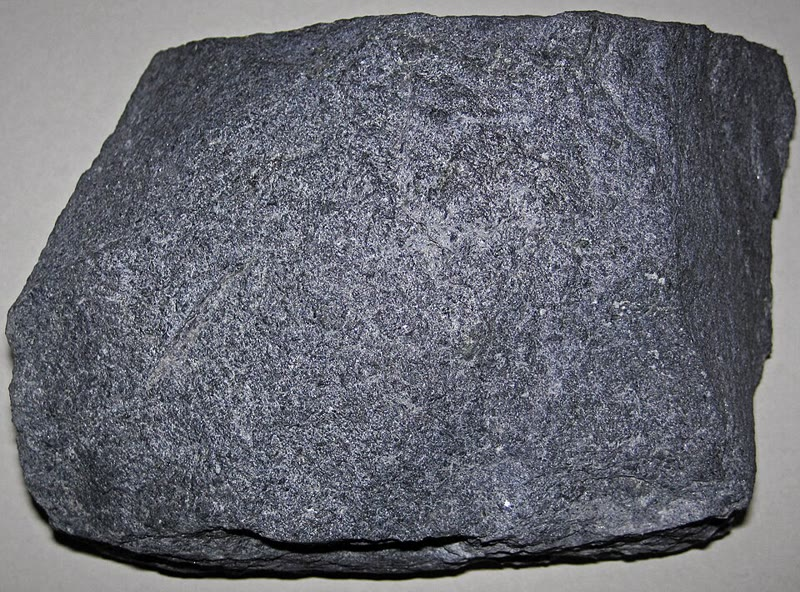
\includegraphics[height=4.4cm]{images/book2/g11-stjohn-blueschist.jpg}\hspace{0.03\linewidth}%
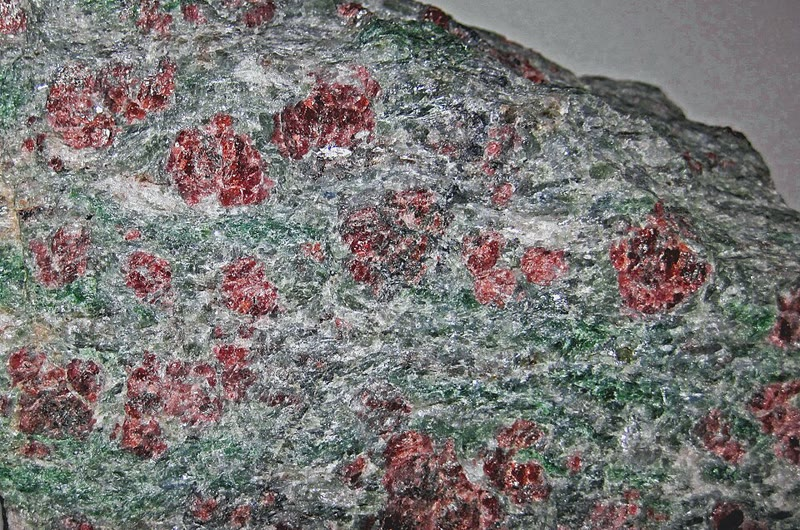
\includegraphics[height=4.4cm]{images/book2/g11-stjohn-eclogite.jpg}

{\small बाएँ: कैलिफ़ोर्निया के सांता कैटालिना द्वीप का \omterm{def:g11:subduction-zones:eclogite}{नीलशिस्ट}, जो कभी किसी \omterm{def:g11:subduction-zones:subduction}{क्षेपण क्षेत्र} में
दबी \omterm{def:g11:ocean-ridges:oceanic-lithosphere}{महासागरीय भूपर्पटी} था। दाएँ: नॉर्वे का \omterm{def:g11:subduction-zones:eclogite}{एक्लोजाइट}, हरे पाइरॉक्सीन में लाल
गार्नेटों के साथ। फ़ोटो जेम्स सेंट~जॉन (CC~BY~2.0)।}
\end{omfigure}
% ledger: photo:g11-blueschist, photo:g11-eclogite

\omterm{def:g11:subduction-zones:eclogite}{एक्लोजाइट} बेसाल्ट से अधिक घना है; यह प्रावार के \omterm{def:g11:ocean-ridges:peridotite}{पेरिडोटाइट} से भी
लगभग \qty{6}{\percent} अधिक घना है। एक बार उसकी भूपर्पटी \omterm{def:g11:subduction-zones:eclogite}{एक्लोजाइट} में बदल जाए,
तो \omterm{def:g11:subduction-zones:slab}{स्लैब} अपने शीर्ष पर कोई हल्की परत नहीं ढोती: पूरी \omterm{def:g11:subduction-zones:slab}{स्लैब} अपने चारों ओर के
प्रावार से अधिक घनी होती है, और अधिक ज़ोर से खींचती है। इस प्रकार की चट्टानें, जिन्हें बाद की गतियाँ
वापस सतह पर ले आईं, \omterm{def:g11:subduction-zones:subduction}{क्षेपण क्षेत्र} में दसियों किलोमीटर नीचे
होने वाली घटनाओं के गिने-चुने प्रत्यक्ष साक्षियों में से हैं।
% ledger: hacker03:eclogite, photo:g11-eclogite

\begin{omfigure}
\begin{tikzpicture}[font=\footnotesize, scale=0.85]
  % subduction zone, a drawing, not to scale: slab top flat to x = -1, then bends to a 42-degree dip
  % coordinates computed once by a small script (scratch, not kept): slab top flat to x=-1, arc R=3 to a 42-degree dip
  \fill[omProp!10] (-7,-1.4) rectangle (7,-6.0);
  \fill[omSea!45] (-7,0) -- (-1,0) -- (1.6,0.8) -- (-7,0.8) -- cycle;
  \fill[lith peridotite] (-7.000,0.000) -- (-6.644,0.000) -- (-6.289,0.000) -- (-5.933,0.000) -- (-5.578,0.000) -- (-5.222,0.000) -- (-4.867,0.000) -- (-4.511,0.000) -- (-4.156,0.000) -- (-3.800,0.000) -- (-3.445,0.000) -- (-3.089,0.000) -- (-2.734,0.000) -- (-2.378,0.000) -- (-2.023,0.000) -- (-1.667,0.000) -- (-1.312,0.000) -- (-0.956,-0.000) -- (-0.602,-0.027) -- (-0.253,-0.094) -- (0.085,-0.203) -- (0.408,-0.351) -- (0.712,-0.536) -- (0.991,-0.756) -- (1.255,-0.994) -- (1.519,-1.232) -- (1.784,-1.470) -- (2.048,-1.707) -- (2.312,-1.945) -- (2.576,-2.183) -- (2.840,-2.421) -- (3.105,-2.659) -- (3.369,-2.897) -- (3.633,-3.135) -- (3.897,-3.373) -- (4.161,-3.611) -- (4.426,-3.848) -- (4.690,-4.086) -- (4.954,-4.324) -- (5.218,-4.562) -- (5.483,-4.800) -- (4.546,-5.840) -- (4.282,-5.603) -- (4.017,-5.365) -- (3.753,-5.127) -- (3.489,-4.889) -- (3.225,-4.651) -- (2.961,-4.413) -- (2.696,-4.175) -- (2.432,-3.937) -- (2.168,-3.699) -- (1.904,-3.461) -- (1.639,-3.224) -- (1.375,-2.986) -- (1.111,-2.748) -- (0.847,-2.510) -- (0.583,-2.272) -- (0.318,-2.034) -- (0.062,-1.803) -- (-0.087,-1.686) -- (-0.249,-1.587) -- (-0.421,-1.508) -- (-0.602,-1.450) -- (-0.788,-1.414) -- (-0.977,-1.400) -- (-1.312,-1.400) -- (-1.667,-1.400) -- (-2.023,-1.400) -- (-2.378,-1.400) -- (-2.734,-1.400) -- (-3.089,-1.400) -- (-3.445,-1.400) -- (-3.800,-1.400) -- (-4.156,-1.400) -- (-4.511,-1.400) -- (-4.867,-1.400) -- (-5.222,-1.400) -- (-5.578,-1.400) -- (-5.933,-1.400) -- (-6.289,-1.400) -- (-6.644,-1.400) -- (-7.000,-1.400) -- cycle;
  \fill[lith basalt] (-7.000,0.000) -- (-6.644,0.000) -- (-6.289,0.000) -- (-5.933,0.000) -- (-5.578,0.000) -- (-5.222,0.000) -- (-4.867,0.000) -- (-4.511,0.000) -- (-4.156,0.000) -- (-3.800,0.000) -- (-3.445,0.000) -- (-3.089,0.000) -- (-2.734,0.000) -- (-2.378,0.000) -- (-2.023,0.000) -- (-1.667,0.000) -- (-1.312,0.000) -- (-0.956,-0.000) -- (-0.602,-0.027) -- (-0.253,-0.094) -- (0.085,-0.203) -- (0.408,-0.351) -- (0.712,-0.536) -- (0.991,-0.756) -- (1.255,-0.994) -- (1.519,-1.232) -- (1.784,-1.470) -- (2.048,-1.707) -- (2.312,-1.945) -- (2.576,-2.183) -- (2.840,-2.421) -- (3.105,-2.659) -- (3.369,-2.897) -- (3.633,-3.135) -- (3.897,-3.373) -- (4.161,-3.611) -- (4.426,-3.848) -- (4.690,-4.086) -- (4.954,-4.324) -- (5.218,-4.562) -- (5.483,-4.800) -- (5.282,-5.023) -- (5.018,-4.785) -- (4.753,-4.547) -- (4.489,-4.309) -- (4.225,-4.071) -- (3.961,-3.833) -- (3.697,-3.596) -- (3.432,-3.358) -- (3.168,-3.120) -- (2.904,-2.882) -- (2.640,-2.644) -- (2.376,-2.406) -- (2.111,-2.168) -- (1.847,-1.930) -- (1.583,-1.692) -- (1.319,-1.455) -- (1.054,-1.217) -- (0.792,-0.980) -- (0.541,-0.783) -- (0.268,-0.616) -- (-0.023,-0.483) -- (-0.328,-0.385) -- (-0.642,-0.324) -- (-0.960,-0.300) -- (-1.312,-0.300) -- (-1.667,-0.300) -- (-2.023,-0.300) -- (-2.378,-0.300) -- (-2.734,-0.300) -- (-3.089,-0.300) -- (-3.445,-0.300) -- (-3.800,-0.300) -- (-4.156,-0.300) -- (-4.511,-0.300) -- (-4.867,-0.300) -- (-5.222,-0.300) -- (-5.578,-0.300) -- (-5.933,-0.300) -- (-6.289,-0.300) -- (-6.644,-0.300) -- (-7.000,-0.300) -- cycle;
  \fill[blue!30] (2.484,-2.100) -- (2.604,-2.208) -- (2.725,-2.317) -- (2.845,-2.425) -- (2.965,-2.533) -- (3.085,-2.642) -- (3.206,-2.750) -- (3.326,-2.858) -- (3.446,-2.967) -- (3.567,-3.075) -- (3.687,-3.183) -- (3.807,-3.292) -- (3.928,-3.400) -- (3.727,-3.623) -- (3.607,-3.515) -- (3.486,-3.406) -- (3.366,-3.298) -- (3.246,-3.190) -- (3.125,-3.081) -- (3.005,-2.973) -- (2.885,-2.865) -- (2.764,-2.756) -- (2.644,-2.648) -- (2.524,-2.540) -- (2.403,-2.431) -- (2.283,-2.323) -- cycle;
  \fill[lith eclogite] (3.928,-3.400) -- (4.057,-3.517) -- (4.187,-3.633) -- (4.316,-3.750) -- (4.446,-3.867) -- (4.576,-3.983) -- (4.705,-4.100) -- (4.835,-4.217) -- (4.964,-4.333) -- (5.094,-4.450) -- (5.223,-4.567) -- (5.353,-4.683) -- (5.483,-4.800) -- (5.282,-5.023) -- (5.152,-4.906) -- (5.023,-4.790) -- (4.893,-4.673) -- (4.764,-4.556) -- (4.634,-4.440) -- (4.504,-4.323) -- (4.375,-4.206) -- (4.245,-4.090) -- (4.116,-3.973) -- (3.986,-3.856) -- (3.857,-3.740) -- (3.727,-3.623) -- cycle;
  \draw[black!60] (-7.000,0.000) -- (-6.644,0.000) -- (-6.289,0.000) -- (-5.933,0.000) -- (-5.578,0.000) -- (-5.222,0.000) -- (-4.867,0.000) -- (-4.511,0.000) -- (-4.156,0.000) -- (-3.800,0.000) -- (-3.445,0.000) -- (-3.089,0.000) -- (-2.734,0.000) -- (-2.378,0.000) -- (-2.023,0.000) -- (-1.667,0.000) -- (-1.312,0.000) -- (-0.956,-0.000) -- (-0.602,-0.027) -- (-0.253,-0.094) -- (0.085,-0.203) -- (0.408,-0.351) -- (0.712,-0.536) -- (0.991,-0.756) -- (1.255,-0.994) -- (1.519,-1.232) -- (1.784,-1.470) -- (2.048,-1.707) -- (2.312,-1.945) -- (2.576,-2.183) -- (2.840,-2.421) -- (3.105,-2.659) -- (3.369,-2.897) -- (3.633,-3.135) -- (3.897,-3.373) -- (4.161,-3.611) -- (4.426,-3.848) -- (4.690,-4.086) -- (4.954,-4.324) -- (5.218,-4.562) -- (5.483,-4.800);
  \draw[black!60] (-7.000,-1.400) -- (-6.644,-1.400) -- (-6.289,-1.400) -- (-5.933,-1.400) -- (-5.578,-1.400) -- (-5.222,-1.400) -- (-4.867,-1.400) -- (-4.511,-1.400) -- (-4.156,-1.400) -- (-3.800,-1.400) -- (-3.445,-1.400) -- (-3.089,-1.400) -- (-2.734,-1.400) -- (-2.378,-1.400) -- (-2.023,-1.400) -- (-1.667,-1.400) -- (-1.312,-1.400) -- (-0.977,-1.400) -- (-0.788,-1.414) -- (-0.602,-1.450) -- (-0.421,-1.508) -- (-0.249,-1.587) -- (-0.087,-1.686) -- (0.062,-1.803) -- (0.318,-2.034) -- (0.583,-2.272) -- (0.847,-2.510) -- (1.111,-2.748) -- (1.375,-2.986) -- (1.639,-3.224) -- (1.904,-3.461) -- (2.168,-3.699) -- (2.432,-3.937) -- (2.696,-4.175) -- (2.961,-4.413) -- (3.225,-4.651) -- (3.489,-4.889) -- (3.753,-5.127) -- (4.017,-5.365) -- (4.282,-5.603) -- (4.546,-5.840);
  \draw[black!60] (5.483,-4.800) -- (4.546,-5.840);
  \fill[omLithGranite!55] (-1.000,0.000) -- (1.600,0.800) -- (7.000,0.800) -- (7.000,-1.600) -- (1.929,-1.600) -- (1.801,-1.485) -- (1.673,-1.370) -- (1.545,-1.255) -- (1.417,-1.140) -- (1.290,-1.025) -- (1.162,-0.910) -- (1.034,-0.795) -- (0.904,-0.682) -- (0.768,-0.577) -- (0.627,-0.479) -- (0.480,-0.390) -- (0.328,-0.310) -- (0.172,-0.238) -- (0.011,-0.176) -- (-0.152,-0.122) -- (-0.318,-0.078) -- (-0.487,-0.044) -- (-0.657,-0.020) -- (-0.828,-0.005) -- (-1.000,0.000) -- cycle;
  \fill[omLithAlluv] (-1.000,0.000) -- (0.550,0.470) -- (0.926,-0.700) -- (0.761,-0.571) -- (0.588,-0.455) -- (0.407,-0.350) -- (0.219,-0.259) -- (0.025,-0.180) -- (-0.174,-0.116) -- (-0.377,-0.065) -- (-0.583,-0.029) -- (-0.791,-0.007) -- (-1.000,0.000) -- cycle;
  \draw[black!60] (-1.000,0.000) -- (1.600,0.800) -- (7.000,0.800) -- (7.000,-1.600) -- (1.929,-1.600) -- (1.801,-1.485) -- (1.673,-1.370) -- (1.545,-1.255) -- (1.417,-1.140) -- (1.290,-1.025) -- (1.162,-0.910) -- (1.034,-0.795) -- (0.904,-0.682) -- (0.768,-0.577) -- (0.627,-0.479) -- (0.480,-0.390) -- (0.328,-0.310) -- (0.172,-0.238) -- (0.011,-0.176) -- (-0.152,-0.122) -- (-0.318,-0.078) -- (-0.487,-0.044) -- (-0.657,-0.020) -- (-0.828,-0.005) -- (-1.000,0.000);
  \draw[omThm!75, densely dashed, line width=0.7pt] (-7.000,-1.150) -- (-6.648,-1.150) -- (-6.296,-1.150) -- (-5.945,-1.150) -- (-5.593,-1.150) -- (-5.241,-1.150) -- (-4.889,-1.150) -- (-4.538,-1.150) -- (-4.186,-1.150) -- (-3.834,-1.150) -- (-3.482,-1.150) -- (-3.130,-1.150) -- (-2.779,-1.150) -- (-2.427,-1.150) -- (-2.075,-1.150) -- (-1.723,-1.150) -- (-1.372,-1.150) -- (-1.020,-1.150) -- (-0.796,-1.161) -- (-0.582,-1.198) -- (-0.374,-1.259) -- (-0.175,-1.344) -- (0.013,-1.452) -- (0.187,-1.581) -- (0.419,-1.788) -- (0.680,-2.023) -- (0.942,-2.259) -- (1.203,-2.494) -- (1.465,-2.730) -- (1.726,-2.965) -- (1.987,-3.200) -- (2.249,-3.436) -- (2.510,-3.671) -- (2.772,-3.907) -- (3.033,-4.142) -- (3.294,-4.377) -- (3.556,-4.613) -- (3.817,-4.848) -- (4.079,-5.083) -- (4.340,-5.319) -- (4.602,-5.554) -- (5.103,-4.997) -- (5.045,-4.944) -- (4.987,-4.892) -- (4.929,-4.839) -- (4.870,-4.787) -- (4.812,-4.734) -- (4.754,-4.682) -- (4.695,-4.629) -- (4.637,-4.577) -- (4.579,-4.524) -- (4.520,-4.472) -- (4.462,-4.419) -- (4.404,-4.367) -- (4.346,-4.315) -- (4.287,-4.262) -- (4.229,-4.210) -- (4.171,-4.157) -- (4.112,-4.105) -- (4.054,-4.052) -- (3.996,-4.000) -- (3.937,-3.947) -- (3.879,-3.895) -- (3.821,-3.842) -- (3.763,-3.790) -- (3.704,-3.737) -- (3.646,-3.685) -- (3.588,-3.632) -- (3.529,-3.580) -- (3.471,-3.527) -- (3.413,-3.475) -- (3.355,-3.422) -- (3.296,-3.370) -- (3.238,-3.317) -- (3.180,-3.265) -- (3.121,-3.212) -- (3.063,-3.160) -- (3.005,-3.107) -- (2.946,-3.055) -- (2.888,-3.002) -- (2.830,-2.950) -- (2.772,-2.897) -- (7.000,-2.897);
  \foreach \p in {(-0.72,-0.22),(-0.46,-0.36),(-0.18,-0.37),(0.05,-0.55),(0.29,-0.67),(0.63,-0.66),(0.87,-0.82),(0.91,-1.23),(1.27,-1.29),(1.50,-1.49),(1.55,-1.89),(1.90,-1.96),(2.04,-2.25),(2.35,-2.36),(2.54,-2.61),(2.88,-2.69),(2.99,-3.02),(3.16,-3.28),(3.47,-3.40),(3.65,-3.66),(3.89,-3.84),(4.26,-3.89),(4.32,-4.27),(4.59,-4.43),(4.88,-4.56),(5.17,-4.70)} \fill[black] \p circle (1.3pt);
  % volcanic arc above the slab, back-arc stretched
  \fill[black!70] (3.35,0.8) -- (3.7,1.4) -- (4.05,0.8) -- cycle;
  \draw[black!45, dashed] (5.2,0.8) -- (5.2,-1.6); \draw[black!45, dashed] (6.6,0.8) -- (6.6,-1.6);
  \draw[{Stealth[length=4pt]}-{Stealth[length=4pt]}, black!70] (5.35,-0.7) -- (6.45,-0.7);
  % motion arrows
  \draw[-{Stealth[length=5pt]}, line width=1pt] (-5.6,0.4) -- (-3.6,0.4);
  \draw[-{Stealth[length=5pt]}, line width=1pt] (1.77,-4.01) -- (2.88,-5.01);
  % labels
  \draw[black!60] (-1.0,0.02) -- (-1.8,1.05);
  \node[anchor=south] at (-1.8,1.05) {खाई};
  \draw[black!60] (0.1,0.12) -- (0.5,1.05);
  \node[anchor=south, align=center] at (0.6,1.05) {खुरचे गए\\अवसाद};
  \node[anchor=south] at (2.35,0.85) {अग्र-चाप};
  \node[anchor=south] at (3.7,1.4) {ज्वालामुखीय चाप};
  \node[anchor=south] at (5.9,0.85) {पश्च-चाप};
  \node[anchor=south] at (-5.4,0.82) {खाई की ओर चलती महासागरीय तली};
  \draw[black!60] (-7.0,-0.15) -- (-7.25,-0.15);
  \node[anchor=east] at (-7.25,-0.15) {महासागरीय भूपर्पटी};
  \draw[black!60] (-7.0,-0.85) -- (-7.25,-0.85);
  \node[anchor=east, align=right] at (-7.25,-0.85) {स्थलमंडल का\\प्रावार-भाग};
  \node at (-3.5,-3.6) {दुर्बलतामंडल};
  \node[rotate=-42] at (3.98,-4.46) {स्लैब};
  \draw[black!60] (3.35,-2.65) -- (4.3,-2.35);
  \node[anchor=west] at (4.3,-2.35) {नीलशिस्ट};
  \draw[black!60] (5.1,-4.3) -- (5.75,-4.6);
  \node[anchor=west] at (5.75,-4.6) {एक्लोजाइट};
  \node[anchor=north east, text=omThm!80!black, align=right] at (7,-2.95) {समान तापमान\\की रेखा};
  \fill[black] (-6.8,-5.55) circle (1.3pt);
  \node[anchor=west] at (-6.65,-5.55) {भूकंप};
\end{tikzpicture}

{\small एक \omterm{def:g11:subduction-zones:subduction}{क्षेपण क्षेत्र} (चित्र, पैमाने पर नहीं)। पुराना \omterm{def:g11:ocean-ridges:oceanic-lithosphere}{महासागरीय स्थलमंडल}
खाई पर नीचे मुड़ता है और ऊपरी प्लेट के नीचे डूबता है। उसकी सतह से
खुरचे गए अवसाद ऊपरी प्लेट के किनारे से सटकर ढेर हो जाते हैं;
भूकंप डूबती \omterm{def:g11:subduction-zones:slab}{स्लैब} का अनुसरण करते हैं; उसकी भूपर्पटी \omterm{def:g11:subduction-zones:eclogite}{नीलशिस्ट} में, फिर
\omterm{def:g11:subduction-zones:eclogite}{एक्लोजाइट} में बदलती है। \omterm{def:g11:subduction-zones:slab}{स्लैब} अपने चारों ओर के प्रावार से ठंडी रहती है: समान
तापमान की रेखाएँ उसके अनुदिश नीचे खिंच जाती हैं। ज्वालामुखियों की एक पंक्ति,
ज्वालामुखीय चाप, \omterm{def:g11:subduction-zones:slab}{स्लैब} के ऊपर खड़ी होती है।}
\end{omfigure}
% volcanic arc above the slab: told only, defined and sourced in g12.04

\section{क्षेपण क्षेत्र की संरचना}

महासागर से महाद्वीप तक, या अगले महासागर तक, \omterm{def:g11:subduction-zones:subduction}{क्षेपण क्षेत्र} के
हमेशा वही भाग होते हैं।

\begin{itemize}
  \item \emph{खाई}, जहाँ डूबती प्लेट नीचे मुड़ती है: महासागरों के सबसे गहरे
        स्थान।
  \item \emph{अग्र-चाप}, खाई और ज्वालामुखियों की पंक्ति के बीच। इसका
        किनारा डूबती प्लेट से खुरचे गए अवसादों का ढेर है; इसके नीचे
        दोनों प्लेटें प्लेट-सीमा के अनुदिश एक-दूसरे के पास से सरकती हैं, जो एक
        मंद झुका हुआ भ्रंश है जिस पर महान भूकंप होते हैं, जैसे
        2011 का जापान के तट के पास का भूकंप (नीचे का उदाहरण)।
  \item \emph{ज्वालामुखीय चाप}, खाई के समांतर ज्वालामुखियों की एक पंक्ति,
        द्वीपों पर (टोंगा, मारियाना, जापान) या किसी महाद्वीप पर (एंडीज़);
        यह क्यों बनता है, यह \cref{ch:g12:subduction-magmatism} का विषय है।
  \item कुछ चापों के पीछे एक \emph{पश्च-चाप}, जहाँ ऊपरी प्लेट
        खिंचती है; टोंगा के पीछे इसे खींचकर अलग किया जा रहा है।
\end{itemize}
% ledger: bevis95:tonga (back-arc extension at Tonga); usgs:tohoku (largest earthquakes on the
% plate boundary: example below)

टोंगा के पीछे पश्च-चाप का खिंचाव स्वयं चाप को प्रशांत
प्लेट की ओर ले जाता है, जैसा उपग्रह-स्थिति-निर्धारण ने दिखाया है। इसलिए जिस दर से टोंगा खाई के दोनों ओर अभिसरित होते हैं,
वह किसी भी प्लेट की अपनी चाल से अधिक है: PB2002 मॉडल से,
\ang{20}~दक्षिण के पास प्रति वर्ष लगभग \qty{17}{cm}।
% values: tonga_rate 168.0 (mean of the PB2002 TO/PA steps within 100 km of the profile);
% PB2002 steps along Tonga: 104 to 237 mm/yr; ledger data:pb2002, bevis95:tonga

\begin{example}[तोहोकु भूकंप, 2011]\label{ex:g11:subduction-zones:tohoku}
11~मार्च 2011 को परिमाण 9.1 का एक भूकंप जापान के होंशू के उत्तर-पूर्वी
तट के पास आया। यह लगभग \qty{25}{km} नीचे, स्वयं प्लेट-सीमा पर हुआ,
जहाँ प्रशांत प्लेट, उत्तरी जापान को ढोने वाली प्लेट के सापेक्ष प्रति वर्ष लगभग \qty{83}{mm}
पश्चिम की ओर चलती हुई, जापान खाई पर उसके नीचे डूबती है। भ्रंश के
दोनों ओर एक-दूसरे के पास से 50 से \qty{60}{m} तक सरके, लगभग \qty{400}{km} लंबे और
\qty{150}{km} चौड़े क्षेत्र पर। ऊपर का समुद्री तल उसके साथ चला, और उसने एक सुनामी उठाई
जो तट पर \qty{38}{m} ऊँचाई तक चढ़ी; कम से कम \num{15703} लोग
मारे गए और \num{4647} लापता हुए। यही तट इस \omterm{def:g11:subduction-zones:subduction}{क्षेपण क्षेत्र} से उठी सुनामियों की
चपेट में 1611, 1896 और 1933 में आया था, और संभवतः वर्ष 869 में 2011 जितनी
बड़ी एक सुनामी की चपेट में भी।
\end{example}
% ledger: usgs:tohoku

\begin{omfigure}
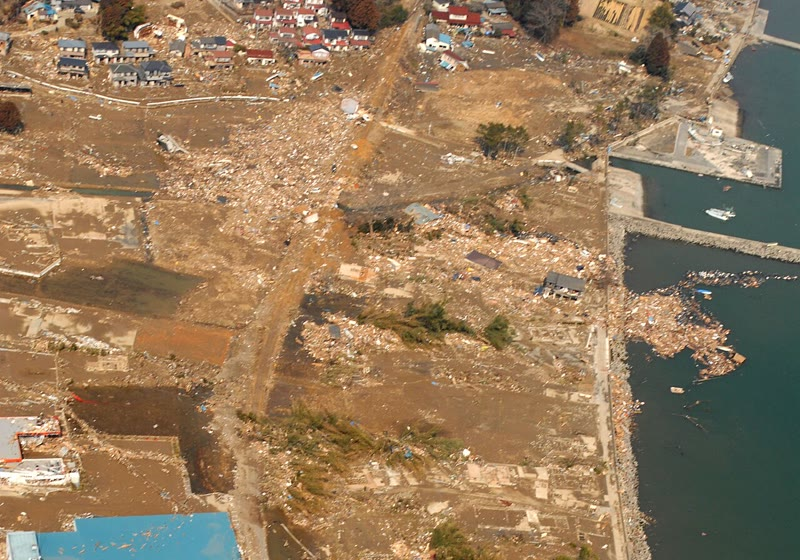
\includegraphics[width=0.78\linewidth]{images/book2/g11-usn-tsunami-kesennuma.jpg}

{\small जापान के उत्तर-पूर्वी तट पर केसेन्नुमा का मत्स्य-बंदरगाह, 11~मार्च 2011 की
सुनामी के दो दिन बाद। फ़ोटो डिलन मैककॉर्ड, अमेरिकी नौसेना
(सार्वजनिक डोमेन)।}
\end{omfigure}
% ledger: photo:g11-tsunami

\section{अभ्यास}

\begin{exercise}[$\star$]\label{exo:g11:subduction-zones:1}
\omterm{def:g11:subduction-zones:subduction}{क्षेपण} और \omterm{def:g11:subduction-zones:subduction}{क्षेपण क्षेत्र} की परिभाषा दीजिए। \omterm{def:g11:subduction-zones:subduction}{क्षेपण क्षेत्र} पर किस प्रकार का \omterm{def:g11:lithosphere-asthenosphere:lithosphere}{स्थलमंडल}
डूबता है, और वही प्रकार क्यों?
\end{exercise}

\begin{exercise}[$\star$]\label{exo:g11:subduction-zones:2}
गहराई के अनुसार भूकंपों के विश्व-मानचित्र का उपयोग कीजिए: (1) ऐसे तीन क्षेत्रों के नाम बताइए जहाँ
\qty{300}{km} से अधिक गहरे भूकंप हैं; (2) गहरे भूकंप खाई की किस ओर
होते हैं? (3) मध्य-अटलांटिक कटक के अनुदिश भूकंप
कितने गहरे होते हैं?
\end{exercise}

\begin{exercise}[$\star$]\label{exo:g11:subduction-zones:3}
सूची में परिमाण 6 या उससे अधिक के \num{7031} भूकंप हैं, जिनमें से
\qty{21}{\percent} \qty{70}{km} से अधिक गहरे हैं और \qty{6.9}{\percent}
\qty{300}{km} से अधिक गहरे। हर स्थिति में यह कितने भूकंप हैं?
\end{exercise}

\begin{exercise}[$\star$]\label{exo:g11:subduction-zones:4}
\omterm{def:g11:subduction-zones:eclogite}{नीलशिस्ट} और \omterm{def:g11:subduction-zones:eclogite}{एक्लोजाइट} की परिभाषा दीजिए। दोनों में \omterm{def:g11:ocean-ridges:oceanic-lithosphere}{महासागरीय भूपर्पटी} के
बेसाल्ट से क्या समान है? क्या भिन्न है?
\end{exercise}

\begin{exercise}[$\star$]\label{exo:g11:subduction-zones:5}
\omterm{def:g11:subduction-zones:subduction}{क्षेपण क्षेत्र} के भागों को क्रम से सूचीबद्ध कीजिए, खाई की ओर चलती
महासागरीय तली से पश्च-चाप तक, और एक पंक्ति में बताइए कि हर एक में
क्या होता है।
\end{exercise}

\begin{exercise}[$\star\star$]\label{exo:g11:subduction-zones:6}
एंडीज़ काट पर भूकंपों का अनुसरण करने वाली रेखा खाई से \qty{300}{km} पर
\qty{135}{km} नीचे से और \qty{800}{km} पर \qty{508}{km} नीचे से
गुज़रती है। \omterm{def:g11:subduction-zones:slab}{स्लैब} का नमन परिकलित कीजिए।
\end{exercise}

\begin{exercise}[$\star\star$]\label{exo:g11:subduction-zones:7}
एक सीधी \omterm{def:g11:subduction-zones:slab}{स्लैब} किसी खाई से शुरू होती है और \ang{45} पर झुकी है। (1) खाई से
\qty{300}{km} पर वह कितनी गहरी है? (2) खाई से किस दूरी पर वह
\qty{670}{km} तक पहुँचती है? (3) खाई और
\qty{670}{km} के बीच \omterm{def:g11:subduction-zones:slab}{स्लैब} की कितनी लंबाई है?
\end{exercise}

\begin{exercise}[$\star\star$]\label{exo:g11:subduction-zones:8}
प्लेटों की माध्य चालें, मिलीमीटर प्रति वर्ष में, ये हैं: कोकोस 74.6, नाज़्का
70.0, प्रशांत 65.5, ऑस्ट्रेलिया 63.1, फ़िलिपीन सागर 52.6 (\omterm{def:g11:subduction-zones:slab}{स्लैब} सहित); अरब
47.6, सोमालिया 31.0, न्यूबिया 29.2, यूरेशिया 22.8, उत्तर अमेरिका 19.8, अंटार्कटिका
15.2, कैरिबियन 14.9, दक्षिण अमेरिका 10.6 (बिना \omterm{def:g11:subduction-zones:slab}{स्लैब})। (1) हर समूह का
माध्य और उनका अनुपात परिकलित कीजिए। (2) इससे प्लेटों को चलाने वाले बल के बारे में
क्या संकेत मिलता है?
\end{exercise}

\begin{exercise}[$\star\star$]\label{exo:g11:subduction-zones:9}
2011 में जापान के तट के पास का भ्रंश 50 से \qty{60}{m} तक सरका।
प्रशांत प्लेट प्रति वर्ष \qty{83}{mm} की दर से पास आती है। (1) \qty{50}{m}, फिर \qty{60}{m}, की सरकन
प्लेट-गति के कितने वर्षों के बराबर है? (2) इसकी तुलना 869 से अब तक के समय से कीजिए,
जो उतने ही आकार का संभावित पहले का भूकंप था।
\end{exercise}

\begin{exercise}[$\star\star$]\label{exo:g11:subduction-zones:10}
जापान खाई तक पहुँचने वाली महासागरीय तली लगभग 133 मिलियन वर्ष पुरानी है,
टोंगा तक पहुँचने वाली लगभग 99 और एंडीज़ तक पहुँचने वाली लगभग 49। (1)
\cref{ch:g11:ocean-ridges} के नियमों ($2500 + 350\sqrt{t}$, जब
$t \le 70$; उसके आगे $6400 - 3200\,e^{-t/62.8}$) का उपयोग करके हर एक की गहराई ज्ञात कीजिए। (2)
सबसे ठंडा और सबसे घना \omterm{def:g11:lithosphere-asthenosphere:lithosphere}{स्थलमंडल} कौन-सा है?
\end{exercise}

\begin{exercise}[$\star\star$]\label{exo:g11:subduction-zones:11}
\omterm{def:g11:ocean-ridges:oceanic-lithosphere}{महासागरीय भूपर्पटी} के बेसाल्ट का घनत्व लगभग \qty{2900}{kg/m^3} है,
\omterm{def:g11:subduction-zones:slab}{स्लैब} के चारों ओर के प्रावार का \qty{3380}{kg/m^3}, और \omterm{def:g11:subduction-zones:eclogite}{एक्लोजाइट}
प्रावार से \qty{6}{\percent} अधिक घना है। (1) \omterm{def:g11:subduction-zones:eclogite}{एक्लोजाइट} का घनत्व ज्ञात कीजिए।
(2) \omterm{def:g11:subduction-zones:eclogite}{एक्लोजाइट} में बदलने पर भूपर्पटी का घनत्व कितने प्रतिशत
बढ़ता है? (3) पहले और बाद में भूपर्पटी प्रावार से हल्की है या घनी, और कितनी?
\end{exercise}

\begin{exercise}[$\star\star\star$]\label{exo:g11:subduction-zones:12}
ऊष्मा चालन द्वारा लगभग $\sqrt{\kappa t}$ की दूरी तक फैलती है,
समय $t$ में, जहाँ चट्टान के लिए $\kappa = \qty{1e-6}{m^2/s}$। (1) 6 मिलियन वर्षों के लिए यह दूरी
परिकलित कीजिए ($1~\text{वर्ष} \approx \qty{3.16e7}{s}$)। (2) इसकी तुलना
किसी \omterm{def:g11:subduction-zones:slab}{स्लैब} की मोटाई, लगभग \qty{100}{km}, से कीजिए। (3) समझाइए कि
\qty{600}{km} पर किसी \omterm{def:g11:subduction-zones:slab}{स्लैब} के भीतर भूकंप क्यों हो सकते हैं जबकि उसके चारों ओर का प्रावार
बहता है।
\end{exercise}
% ledger: england:kelvin (kappa 1e-6 m2/s)

\begin{exercise}[$\star\star\star$]\label{exo:g11:subduction-zones:13}
\ang{21}~दक्षिण पर एंडीज़ के नीचे काट की रेखा खाई से \qty{1017}{km} पर
\qty{670}{km} तक पहुँचती है, और प्लेटें प्रति वर्ष
\qty{64}{mm} की दर से अभिसरित होती हैं। (1) खाई से \qty{670}{km} तक \omterm{def:g11:subduction-zones:slab}{स्लैब} की लंबाई का
अनुमान लगाइए। (2) महासागरीय तली के किसी टुकड़े को
\qty{670}{km} तक पहुँचने में कितना समय लगता है? (3) टोंगा से तुलना कीजिए, जहाँ यही यात्रा लगभग 6
मिलियन वर्ष लेती है।
\end{exercise}

\begin{exercise}[$\star\star\star$]\label{exo:g11:subduction-zones:14}
किसी खाई के नीचे एक \omterm{def:g11:subduction-zones:slab}{स्लैब} लीजिए, \qty{100}{km} मोटी, अपने चारों ओर के प्रावार से
औसतन \qty{36}{kg/m^3} अधिक घनी, और \qty{1000}{km} लंबी।
(1) खाई के हर मीटर के लिए \omterm{def:g11:subduction-zones:slab}{स्लैब} का अतिरिक्त द्रव्यमान परिकलित कीजिए। (2)
$g = \qty{9.8}{m/s^2}$ के साथ उसका भार परिकलित कीजिए। (3) यह बल पूरी
प्लेट को क्यों खींच सकता है?
\end{exercise}

\begin{exercise}[$\star\star\star$]\label{exo:g11:subduction-zones:15}
टोंगा खाई के अनुदिश PB2002 मॉडल \ang{23.6}~दक्षिण पर प्रति वर्ष \qty{104}{mm}
और \ang{16.5}~दक्षिण पर प्रति वर्ष \qty{237}{mm} का अभिसरण देता है। (1) किसी याम्योत्तर के
अनुदिश दोनों बिंदु कितनी दूर हैं
($\ang{1} \approx \qty{111}{km}$)? (2) प्रति सौ किलोमीटर दर कितनी
बढ़ती है? (3) प्रशांत प्लेट दोनों बिंदुओं पर लगभग एक ही चाल से चलती है।
खाई की दूसरी ओर, यानी टोंगा चाप, को क्या करना चाहिए?
\end{exercise}

\section{समस्या: टोंगा स्लैब}

\begin{problem}[{सप्ताहांत समस्या --- खाई से \qty{670}{km} तक}]
\label{pb:g11:subduction-zones:1}
% values: tonga fit -23.568 + 0.91068 x; tonga_rate 168.0 mm/yr; tonga_age 98.8;
% x670 761.6; path 1014; time 6.04 Myr; tonga_maxdepth 670.8 (slab_sections.py);
% MKEA 69 mm/yr (plate_velocities.py); kappa england:kelvin; eclogite hacker03:eclogite
टोंगा खाई के नीचे प्रशांत प्लेट पश्चिम की ओर डूबती है। इस अध्याय की टोंगा
काट का उपयोग कीजिए, जिसकी रेखा $z = -24 + 0.91\,x$ है (दोनों
किलोमीटर में, $x$ खाई से चाप की ओर मापा गया)।

\medskip
\noindent\textbf{भाग I --- भूकंप-काट।}
\begin{enumerate}
  \item काट का सबसे गहरा भूकंप कितना गहरा है?
  \item खाई की महासागर वाली ओर गहरे भूकंप क्यों नहीं हैं?
  \item $x = 300$ और $x = 700$ पर रेखा की गहराई परिकलित कीजिए, फिर
        \omterm{def:g11:subduction-zones:slab}{स्लैब} का नमन।
  \item खाई से किस क्षैतिज दूरी पर \omterm{def:g11:subduction-zones:slab}{स्लैब}
        \qty{100}{km} गहरी है? और \qty{400}{km} गहरी?
  \item $x = 0$ पर रेखा खाई से \qty{24}{km} ऊपर से गुज़रती है। इससे
        खाई के पास \omterm{def:g11:subduction-zones:slab}{स्लैब} के आकार के बारे में क्या पता चलता है?
\end{enumerate}

\medskip
\noindent\textbf{भाग II --- अभिसरण।}
\begin{enumerate}[resume]
  \item प्लेटें खाई के आर-पार प्रति वर्ष लगभग \qty{168}{mm} की दर से अभिसरित होती हैं।
        इसे सेंटीमीटर प्रति वर्ष और किलोमीटर प्रति मिलियन वर्ष में बदलिए।
  \item प्रशांत प्लेट हवाई के ऊपर से प्रति वर्ष लगभग \qty{69}{mm} चलती है।
        टोंगा पर अभिसरण कितने गुना तेज़ है?
  \item सापेक्ष वेगों के योग का उपयोग करके समझाइए कि अभिसरण
        प्रशांत प्लेट की चाल से अधिक कैसे हो सकता है।
  \item खाई तक पहुँचने वाली तली लगभग 99 मिलियन वर्ष पुरानी है। वह कितनी
        गहराई पर है (\cref{ch:g11:ocean-ridges} का चरघातांकी नियम)?
  \item ऐसा \omterm{def:g11:lithosphere-asthenosphere:lithosphere}{स्थलमंडल} अपने आप क्यों डूब सकता है?
\end{enumerate}

\medskip
\noindent\textbf{भाग III --- \qty{670}{km} तक नीचे।}
\begin{enumerate}[resume]
  \item खाई से किस क्षैतिज दूरी पर रेखा
        \qty{670}{km} तक पहुँचती है?
  \item \omterm{def:g11:subduction-zones:slab}{स्लैब} को सीधी मानकर खाई से उस बिंदु तक उसकी लंबाई का
        अनुमान लगाइए।
  \item महासागरीय तली के किसी टुकड़े को प्रति वर्ष \qty{168}{mm} पर यह लंबाई
        तय करने में कितना समय लगता है?
  \item हवाई के ऊपर प्रशांत प्लेट की प्रति वर्ष \qty{69}{mm} की चाल पर इसमें कितना
        समय लगता?
  \item रास्ते में \omterm{def:g11:subduction-zones:slab}{स्लैब} की भूपर्पटी \omterm{def:g11:subduction-zones:eclogite}{एक्लोजाइट} में बदल जाती है, जो
        \qty{3380}{kg/m^3} वाले प्रावार से \qty{6}{\percent} अधिक घना है। उसका
        घनत्व क्या है, और इससे \omterm{def:g11:subduction-zones:slab}{स्लैब} के लिए क्या बदलता है?
\end{enumerate}

\medskip
\noindent\textbf{भाग IV --- गरम प्रावार में एक ठंडी स्लैब।}
\begin{enumerate}[resume]
  \item प्रश्न~13 के समय में ऊष्मा चालन द्वारा लगभग
        $\sqrt{\kappa t}$ तक फैलती है, जहाँ $\kappa = \qty{1e-6}{m^2/s}$। यह
        दूरी परिकलित कीजिए।
  \item इसकी तुलना \omterm{def:g11:subduction-zones:slab}{स्लैब} की मोटाई, लगभग \qty{100}{km}, से कीजिए। क्या
        \qty{670}{km} तक पहुँचने पर \omterm{def:g11:subduction-zones:slab}{स्लैब} भीतर से अब भी ठंडी है?
  \item इससे टोंगा के नीचे \qty{600}{km} और उससे अधिक पर के भूकंप
        कैसे समझ में आते हैं?
  \item भूकंपीय तरंगों ने \qty{670}{km} के पास प्रावार में कौन-सा परिवर्तन
        प्रकट किया (\cref{ch:g11:seismic-structure})?
  \item निष्कर्ष निकालिए: प्रशांत महासागरीय तली को टोंगा
        खाई से \qty{670}{km} तक नीचे जाने में कितना समय लगता है?
\end{enumerate}
\end{problem}
